% Drawing 156-6/04-2 -- folder 156-6, batch 04, archive page 73 (PDF page 74).
% Transcription: schéma (barré) : un hexagone $F, H, G$ en haut, $F', K', G'$ en bas, avec $K$ et $H'$ au centre ; flèches à crochet pour les $\leq$ ($F \to H$, $G \to H$, $K \to F$, $K \to G$, $K' \to F'$, $K' \to G'$, $F' \to H'$, $G' \to H'$) et flèches verticales pour les $\ll$ ($F' \to F$, $G' \to G$, $H' \to H$, $K' \to K$). Il est repris au propre page 74
% Kind: struck hexagon of inclusions F, H, G / F', K', G' with K, H' in the centre. Method 2 (schematic redraw from the facsimile). Status: ok.
% Notes: Struck diagram (three long oblique strokes cross it, drawn grey): F, H, G at the top, F', K', G' at the bottom, K and H' in the centre; arrows for <= (F -> H, G -> H, K -> F, K -> G, K' -> F', K' -> G', F' -> H', G' -> H') and upward arrows for << (F' -> F, G' -> G, H' -> H, K' -> K). Hooked arrows (for <=) are drawn as plain arrows, vertical arrows (for <<) likewise; the kind of arrow is said here.
% Coordinates: 1 unit = 1 mm = 1/100 of the crop width (bbox in page fractions: [0.18, 0.54, 0.52, 0.69]).
% Redrawn by Claude (claude-opus-5-5), issue #73, 2026-11-07; not checked by a human; not compiled (no TeX in the session).
% Rights: reproduces part of the work -- behind RENDER_TRANSCRIPTS, never published by itself.
\documentclass[tikz,border=3pt]{standalone}
\usepackage{amsmath,amssymb}
\usetikzlibrary{patterns,arrows.meta}
\tikzset{pencil/.style={black!45}, struck/.style={black!35}, mark/.style={circle,draw,inner sep=1.3pt}, pt/.style={circle,fill,inner sep=0.9pt}, opt/.style={circle,draw,fill=white,inner sep=1.1pt}}
\begin{document}
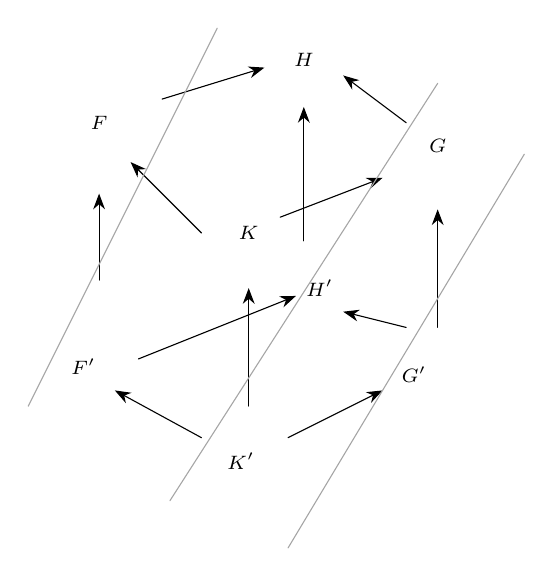
\begin{tikzpicture}[x=1mm,y=1mm,line cap=round,line join=round,font=\scriptsize]
\node[inner sep=1pt] at (43,-14) {\scriptsize $F$};
\node[inner sep=1pt] at (69,-6) {\scriptsize $H$};
\node[inner sep=1pt] at (86,-17) {\scriptsize $G$};
\node[inner sep=1pt] at (62,-28) {\scriptsize $K$};
\node[inner sep=1pt] at (71,-35) {\scriptsize $H'$};
\node[inner sep=1pt] at (41,-45) {\scriptsize $F'$};
\node[inner sep=1pt] at (83,-46) {\scriptsize $G'$};
\node[inner sep=1pt] at (61,-57) {\scriptsize $K'$};
\draw[-{Stealth[length=2mm]}] (51,-11) -- (64,-7);
\draw[-{Stealth[length=2mm]}] (82,-14) -- (74,-8);
\draw[-{Stealth[length=2mm]}] (56,-28) -- (47,-19);
\draw[-{Stealth[length=2mm]}] (66,-26) -- (79,-21);
\draw[-{Stealth[length=2mm]}] (56,-54) -- (45,-48);
\draw[-{Stealth[length=2mm]}] (67,-54) -- (79,-48);
\draw[-{Stealth[length=2mm]}] (48,-44) -- (68,-36);
\draw[-{Stealth[length=2mm]}] (82,-40) -- (74,-38);
\draw[-{Stealth[length=2mm]}] (43,-34) -- (43,-23);
\draw[-{Stealth[length=2mm]}] (86,-40) -- (86,-25);
\draw[-{Stealth[length=2mm]}] (69,-29) -- (69,-12);
\draw[-{Stealth[length=2mm]}] (62,-50) -- (62,-35);
\draw[struck] (34,-50) -- (58,-2);
\draw[struck] (52,-62) -- (86,-9);
\draw[struck] (67,-68) -- (97,-18);
\end{tikzpicture}
\end{document}
